% RITMO - User Manual
%
% Built with XeLaTeX by build.sh (make-screenshots.sh makes the images from the program, md2tex.py
% the generated/*.tex fragments from the Markdown documents of doc/).
\documentclass[11pt,a4paper,oneside,openany]{book}

\usepackage[a4paper,margin=2.4cm,bottom=2.8cm]{geometry}
\usepackage{fontspec}
\setmainfont{Latin Modern Roman}
\setsansfont{Fira Sans}
\setmonofont{DejaVu Sans Mono}[Scale=MatchLowercase]
\usepackage{microtype}
\usepackage{xcolor}
\usepackage{graphicx}
\usepackage{float}
\usepackage{caption}
\usepackage{booktabs}
\usepackage{longtable}
\usepackage{array}
\usepackage{calc}
\usepackage{enumitem}
\usepackage{titlesec}
\usepackage{fancyhdr}
\usepackage{tcolorbox}
\usepackage{listings}
\usepackage[hidelinks]{hyperref}
\usepackage{bookmark}

% the colours of the logo
\definecolor{ritmoblue}{HTML}{0A0A28}
\definecolor{ritmoorange}{HTML}{FF6A2C}
\definecolor{ritmoyellow}{HTML}{FFD23C}
\definecolor{ritmomagenta}{HTML}{C63CC4}
\definecolor{ritmosky}{HTML}{3F8FD0}

\hypersetup{pdftitle={RITMO - User Manual},pdfauthor={RITMO contributors},
  pdfsubject={Atari POKEY music tracker},colorlinks=true,linkcolor=ritmosky!70!black,
  urlcolor=ritmosky!70!black}

\setlength{\parindent}{0pt}
\setlength{\parskip}{0.55em}
\setlist{itemsep=0.15em,topsep=0.3em}
\renewcommand{\arraystretch}{1.15}
\setlength{\emergencystretch}{3em}

% pandoc fragments
\providecommand{\tightlist}{\setlength{\itemsep}{0pt}\setlength{\parskip}{0pt}}
\newcommand{\passthrough}[1]{#1}

% chapter and section titles
\titleformat{\chapter}[display]
  {\sffamily\bfseries\color{ritmoblue}}{\large\color{ritmoorange}\MakeUppercase{\chaptertitlename}\ \thechapter}{0.3em}
  {\Huge}[\vspace{0.3em}{\color{ritmoorange}\titlerule[2pt]}]
\titleformat{\section}{\sffamily\Large\bfseries\color{ritmoblue}}{\thesection}{0.7em}{}
\titleformat{\subsection}{\sffamily\large\bfseries\color{ritmoblue}}{\thesubsection}{0.7em}{}
\titleformat{\subsubsection}{\sffamily\normalsize\bfseries\color{ritmoblue}}{\thesubsubsection}{0.7em}{}
\titlespacing*{\chapter}{0pt}{-10pt}{22pt}

\pagestyle{fancy}
\fancyhf{}
\fancyhead[L]{\sffamily\small\leftmark}
\fancyhead[R]{\sffamily\small RITMO}
\fancyfoot[C]{\sffamily\small\thepage}
\renewcommand{\headrulewidth}{0.3pt}
\fancypagestyle{plain}{\fancyhf{}\fancyfoot[C]{\sffamily\small\thepage}\renewcommand{\headrulewidth}{0pt}}

\captionsetup{font={small,sf},labelfont={bf,color=ritmoorange},labelsep=period}

% a screenshot: \shot{file}{caption}{width as a fraction of the text width}
\newcommand{\shot}[3]{%
  \begin{figure}[H]\centering
    \fbox{\includegraphics[width=#3\textwidth]{images/#1.png}}%
    \caption{#2}\label{fig:#1}%
  \end{figure}}
% a pixel of the screenshots: they have 96 dpi (Qt 6 writes it in the PNG), so a pixel is 72/96 bp
\newlength{\screenpx}
\setlength{\screenpx}{0.75bp}
% a part of a screenshot, enlarged: \shotpart{file}{caption}{width as a fraction of the text width}
% {left}{bottom}{right}{top}, what is cut away on each side, in pixels of the screenshot
\newcommand{\shotpart}[7]{%
  \begin{figure}[H]\centering
    \fbox{\includegraphics[width=#3\textwidth,trim=#4\screenpx{} #5\screenpx{} #6\screenpx{} #7\screenpx,clip]{images/#1.png}}%
    \caption{#2}\label{fig:#1}%
  \end{figure}}
% a screenshot of a dialog, at its own size: \dialog{file}{caption}{width in cm}
\newcommand{\dialog}[3]{%
  \begin{figure}[H]\centering
    \fbox{\includegraphics[width=#3]{images/#1.png}}%
    \caption{#2}\label{fig:#1}%
  \end{figure}}

% names and keys
\newcommand{\key}[1]{\texttt{\small #1}}
\newcommand{\menu}[1]{\textsf{\textbf{#1}}}
\newcommand{\RITMO}{\textsf{RITMO}}
\newcommand{\RMT}{\textsf{RMT}}

\newtcolorbox{note}[1][Note]{colback=ritmoyellow!12,colframe=ritmoorange!80,fonttitle=\sffamily\bfseries,title=#1,
  boxrule=0.6pt,arc=2pt,left=6pt,right=6pt,top=4pt,bottom=4pt}
\newtcolorbox{tip}[1][Tip]{colback=ritmosky!8,colframe=ritmosky!80,fonttitle=\sffamily\bfseries,title=#1,
  boxrule=0.6pt,arc=2pt,left=6pt,right=6pt,top=4pt,bottom=4pt}

\lstset{basicstyle=\ttfamily\small,backgroundcolor=\color{black!4},frame=single,rulecolor=\color{black!20},
  breaklines=true,columns=fullflexible,keepspaces=true,xleftmargin=2pt,xrightmargin=2pt,
  literate={Š}{{\v{S}}}1}

\input{generated/version.tex}

\begin{document}

% ---------------------------------------------------------------- title page
\begin{titlepage}
  \centering
  \vspace*{1.2cm}
  \includegraphics[width=\textwidth]{../logo/ritmo-logo.png}\par
  \vspace{1.4cm}
  {\sffamily\bfseries\fontsize{34}{40}\selectfont\color{ritmoblue} User Manual\par}
  \vspace{0.6cm}
  {\sffamily\Large Version \RitmoVersion\par}
  \vspace{2.2cm}
  {\sffamily\large
  A music tracker for the POKEY sound chip\\of the Atari 8-bit computers (XL/XE)\par}
  \vfill
  {\small Based on RASTER Music Tracker by Radek \v{S}t\v{e}rba (R.I.P.), VinsCool and Peter Dell (JAC!)\\[0.4em]
  \RitmoDate\par}
\end{titlepage}

\frontmatter
\chapter*{About this manual}
\addcontentsline{toc}{chapter}{About this manual}

This manual describes \RITMO{}, a music tracker for the POKEY sound chip of the Atari XL/XE
8-bit computers. \RITMO{} (\emph{\RITMO{} Is a Tracker for Music On Atari}) is a fork of the
RASTER Music Tracker (\RMT{}), and runs on Linux, Windows and macOS.

It is written for two kinds of reader: the musician who wants to compose, and the Atari
programmer who wants to use the result in a demo or a game. Chapters~\ref{ch:intro} to
\ref{ch:tutorial} introduce the program and walk through a first song; the next ones describe
every part of the window, the menus, the dialogs, the import and export formats, MIDI input
and the scripting; the appendices are the complete reference of the keys, the fields and the
file format.

\section*{Conventions}

\begin{itemize}
  \item Keys are written like \key{CONTROL+S} or \key{F5}. \key{CONTROL} is the \key{Ctrl} key
        (on macOS the \key{Control} key, not \key{Command}).
  \item A menu item is written \menu{File $\rightarrow$ Open\ldots}.
  \item Hexadecimal numbers have a \texttt{\$} in front: \texttt{\$3F} is 63. The tracker shows
        its numbers in hexadecimal: line numbers, instruments, volumes.
  \item The names of the fields of the screen are written as the program writes them, in capital
        letters: \texttt{VOLUME}, \texttt{TABLE LENGTH}.
  \item The screenshots are taken from the program itself, by the script
        \texttt{doc/\allowbreak manual/\allowbreak make-\allowbreak screenshots.sh}, with the default settings of a first start
        and the same font on every computer.
\end{itemize}

\begin{note}[RMT and RITMO in the reference]
The reference tables are converted from the documents of the original \RMT{}, and still call the program \RMT{} in places. \RMT{} is also the name of
the file format and of the player routines: an \emph{RMT module} and the \emph{RMT drivers} keep their names in \RITMO{}.
\end{note}

\begin{note}[Where the reference tables come from]
The tables of the menu commands, of the note keys, of the scripting commands and of the tracker
drivers (appendix~\ref{app:reference} and chapters~\ref{ch:drivers} and~\ref{ch:scripting}) are
converted from the Markdown documents in the \texttt{doc/} folder of the program, and the menu and note key
tables of those are written by the program itself (the \texttt{dump actions} and
\texttt{dump notekeys} script commands). They are always the state of the version this manual
is built from.
\end{note}

\tableofcontents

\mainmatter
\chapter{Introduction}\label{ch:intro}

\section{What \RITMO{} is}

The Atari XL/XE computers make their sound with the POKEY chip: four independent voices
(sixteen when two chips are used, as in many stereo songs), each with a frequency divider, a
choice of noise and tone distortions and a volume. A \emph{tracker} is the kind of music editor
that was born on the Amiga: the music is a grid of numbers, one column for each voice and one
row for each beat, and the notes are typed with the computer keyboard as on a piano.

\RITMO{} is such a tracker for the POKEY. A song made with it can be played on a real Atari: the
program produces the same data the player routines of the Atari read, and exports them in
several formats (a SAP file for the Atari players, an executable \texttt{.xex}, assembler source,
the compact RMT module for your own program). The sound you hear while composing comes from an
emulation of the Atari's 6502 processor and of the POKEY chip built into the program, running
the same player routine, so it is what the Atari will play.

\shot{window-tracks}{The main window of \RITMO{} with a song loaded.}{0.98}

\section{History}

\RITMO{} is a fork of the \emph{RASTER Music Tracker}, \RMT{}. The first version, 1.0, was
written by Radek \v{S}t\v{e}rba (Raster/C.P.U.) in 2002; his last version is 1.28, of 2009. It was
a small revolution for the Atari musicians: the first tracker for the POKEY with a
graphical envelope editor, and the one nearly everybody used. Radek \v{S}t\v{e}rba has since
passed away; this manual is, among other things, a way to remember his work. R.I.P.

Vin Samuel (\emph{VinsCool}) continued the program from 2021 to 2024, up to the version 1.34: a
new player routine with more tuning tables, a tuning calculator, an automatic high pass filter,
the SAP and XEX export and many corrections. Peter Dell (\emph{JAC!}) carries on the original
project from 2024 (version 1.35 and the planned version 2) and made it possible for this fork
to exist: everything described here is built on his work.

The \RITMO{} fork keeps the code of the tracker, the file formats and the player routines of
\RMT{} 1.35, and replaces what tied it to Windows. It is renamed so that it cannot be confused with the original
\RMT{}, and so that the Windows-only (MFC) parts of the code could be removed.

\section{What is different from \RMT{}}

\begin{itemize}
  \item The program is written with Qt: it runs natively on Linux, on Windows and on macOS (Intel and
        Apple Silicon). The look of the tracker screen is the original one, pixel for pixel.
  \item The 6502 and the POKEY emulations are built in: the \texttt{sa\_c6502.dll} and
        \texttt{apokeysnd.dll} libraries of the Windows versions are not needed any more.
  \item The sound goes out through PortAudio, and the MIDI input comes in through RtMidi.
  \item The configuration is kept per user in the settings of the system, not in an \texttt{.ini}
        file next to the program. The settings of \RMT{} are taken over at the first start.
  \item Songs, instruments and tracks are the same files as in \RMT{} 1.3x: you can move your work
        between the programs. The files keep their extensions, \texttt{.rmt} and the others.
\end{itemize}

\section{Files used by \RITMO{}}

\begin{center}
\begin{tabular}{@{}>{\raggedright\arraybackslash}p{3.6cm}p{10.4cm}@{}}
\toprule
Extension & Content \\ \midrule
\texttt{.rmt} & an RMT module: the song, its tracks and its instruments (and, if the song was saved
                with \menu{Save}, the names of the song and of the instruments) \\
\texttt{.txt} & the same song as a text file, which can be read and edited with any editor; a single track is saved as a text file too \\
\texttt{.rmw} & a song work file: an RMT module with the state of the editing \\
\texttt{.rti} & a single instrument \\
\texttt{.sap}, \texttt{.sapr}, \texttt{.xex}, \texttt{.asm}, \texttt{.wav}, \texttt{.lzss} & the exported formats (chapter~\ref{ch:importexport}) \\
\texttt{.mod}, \texttt{.tmc}, \texttt{.tm8} & the formats that can be imported \\
\texttt{.rmtscript} & a script (chapter~\ref{ch:scripting}) \\
\bottomrule
\end{tabular}
\end{center}

\chapter{Installing and starting}\label{ch:install}

\section{The packages}

Everything the program needs is inside each package: the tracker drivers and the other files it
loads at run time are in the \texttt{resources} folder next to the program. (The \texttt{.deb} of
riscv64, ppc64 and ppc64le asks the package manager for the libraries instead of carrying them,
section~\ref{sec:linux-arch}.)

\begin{center}
\begin{tabular}{@{}>{\raggedright\arraybackslash}p{3.0cm}>{\raggedright\arraybackslash}p{4.6cm}>{\raggedright\arraybackslash}p{6.2cm}@{}}
\toprule
System & Package & How to start it \\ \midrule
Linux x86\_64 (Debian 11, Ubuntu 20.04 and newer) & \texttt{Ritmo-}\emph{version}\texttt{-\allowbreak x86\_64.AppImage} &
  make it executable (\texttt{chmod +x}) and run it \\
Windows 64 bit & \texttt{Ritmo-Windows-x64-Setup-}\emph{version}\texttt{.exe}, \texttt{Ritmo-Windows-x64-}\emph{version}\texttt{.zip} &
  run the installer (it asks whether to install for all the users or for the current one, and offers a desktop icon and the
  \texttt{.rmt} file type), or unzip the archive anywhere and run \texttt{Ritmo.exe} (the program is not signed: Windows may ask to confirm) \\
macOS 12 or later, Apple Silicon or Intel & \texttt{Ritmo-macOS-arm64-}\emph{version}\texttt{.dmg}, \texttt{Ritmo-macOS-x86\_64-}\emph{version}\texttt{.dmg} &
  drag \texttt{Ritmo.app} to Applications; the first time open it with the right button and
  \menu{Open} (the program is not signed) \\
Linux aarch64: Raspberry Pi 3/4/5 with a 64 bit system (Raspberry Pi OS 13, Debian 13, Ubuntu 24.04 and newer) &
  \texttt{Ritmo-}\emph{version}\texttt{-\allowbreak aarch64.AppImage} & as the x86\_64 one \\
Linux riscv64 (Debian 13 and newer) & \texttt{Ritmo-}\emph{version}\texttt{-\allowbreak riscv64.AppImage}, \texttt{ritmo\_}\emph{version}\texttt{\_riscv64.deb}, \texttt{Ritmo-Linux-\allowbreak riscv64-}\emph{version}\texttt{.tar.gz} &
  run the AppImage, install the \texttt{.deb} with \texttt{apt}, or unpack the archive (section~\ref{sec:linux-arch}) \\
Linux ppc64: PowerPC 64 bit big endian (Debian ports, \emph{sid}) & \texttt{Ritmo-}\emph{version}\texttt{-\allowbreak ppc64.AppImage}, \texttt{ritmo\_}\emph{version}\texttt{\_ppc64.deb}, \texttt{Ritmo-Linux-\allowbreak ppc64-}\emph{version}\texttt{.tar.gz} &
  as riscv64 \\
Linux ppc64le: PowerPC 64 bit little endian, POWER8 and newer (Debian 13 and newer) & \texttt{Ritmo-}\emph{version}\texttt{-\allowbreak ppc64le.AppImage}, \texttt{ritmo\_}\emph{version}\texttt{\_ppc64el.deb}, \texttt{Ritmo-Linux-\allowbreak ppc64el-}\emph{version}\texttt{.tar.gz} &
  as riscv64 (from 2.6) \\
\bottomrule
\end{tabular}
\end{center}

\RITMO{} can also be built from the source with CMake and Qt (appendix~\ref{app:building}).

\begin{note}
The packages of the versions up to 2.2.1 were called \texttt{RMT-*} and the program \texttt{rmt}
(\texttt{Rmt.exe}). From the next releases the packages are \texttt{Ritmo-*} and the program
\texttt{ritmo} (\texttt{Ritmo.exe}). From 2.6 their names carry the version, so that several can be kept side by side:
\emph{version} is \texttt{2.6} for the release 2.6, \texttt{2.6-rc3} for a test build; up to 2.5 the names had no
version (\texttt{Ritmo-Linux-x86\_64.AppImage}); from 2.6 the AppImage has no \texttt{Linux} in its name
(\texttt{Ritmo-2.6-x86\_64.AppImage}) and can update itself with AppImageUpdate. The examples of this chapter use \texttt{2.6}.
\end{note}

\section{Linux, architecture by architecture}\label{sec:linux-arch}

\texttt{uname -m} tells the architecture of the machine: \texttt{x86\_64}, \texttt{aarch64}, \texttt{riscv64}, \texttt{ppc64} or
\texttt{ppc64le} (whose Debian name, in the \texttt{.deb} and the \texttt{.tar.gz}, is \texttt{ppc64el}).

\subsection{x86\_64 and aarch64 (Raspberry Pi): the AppImage}

An AppImage is one file with the program and everything it needs (Qt, PortAudio, RtMidi). It only needs the
\texttt{libfuse2} library to start (on Debian 13 and Ubuntu 24.04 the package is called \texttt{libfuse2t64}):
\begin{lstlisting}
sudo apt install libfuse2                  # libfuse2t64 on Debian 13 and Ubuntu 24.04
chmod +x Ritmo-2.6-x86_64.AppImage   # Raspberry Pi: Ritmo-2.6-aarch64.AppImage
./Ritmo-2.6-x86_64.AppImage mysong.rmt
\end{lstlisting}
Without FUSE the file can still run, unpacking itself in a temporary folder:
\begin{lstlisting}
./Ritmo-2.6-x86_64.AppImage --appimage-extract-and-run mysong.rmt
\end{lstlisting}
The x86\_64 AppImage runs on Debian 11, Ubuntu 20.04 and newer. The aarch64 one needs glibc 2.38 or newer: Raspberry Pi OS 13
(\emph{trixie}), Debian 13, Ubuntu 24.04 and newer, on a Raspberry Pi 3, 4 or 5 with a 64 bit system (\texttt{uname -m} must say
\texttt{aarch64}: on a 32 bit system it says \texttt{armv7l} and there is no package).

\subsection{riscv64, ppc64 and ppc64le: the AppImage}

From 2.6 these architectures have an AppImage too, started as the x86\_64 one:
\begin{lstlisting}
sudo apt install fuse3                     # FUSE for the AppImage
chmod +x Ritmo-2.6-riscv64.AppImage        # Ritmo-2.6-ppc64.AppImage, Ritmo-2.6-ppc64le.AppImage
./Ritmo-2.6-riscv64.AppImage mysong.rmt
./Ritmo-2.6-riscv64.AppImage --appimage-extract-and-run mysong.rmt   # without FUSE
\end{lstlisting}
It carries the same files as the archive below: Qt~6, PortAudio and RtMidi, but not glibc and the graphics and sound
libraries of the drivers, so it needs the same Debian releases and the packages that the \texttt{README.txt} of the archive
lists. There is no official \texttt{appimagetool} for these architectures yet: the AppImages are made with its ports to
riscv64, ppc64 and ppc64le and to their runtimes (\url{https://github.com/gianlucarenzi/appimagetool},
\url{https://github.com/gianlucarenzi/type2-runtime}), proposed to the AppImage project.

\subsection{riscv64, ppc64 and ppc64le: the .deb}

For Debian and the systems derived from it, riscv64 and ppc64le (PowerPC 64 bit \emph{little endian}, POWER8 and newer) need
Debian 13 or newer, and ppc64 (PowerPC 64 bit \emph{big endian}) the \emph{sid} release of Debian ports, the only one that has
this architecture. The \texttt{.deb} contains the program and
\texttt{apt} installs the libraries it needs (Qt~6, PortAudio, RtMidi...) by itself:
\begin{lstlisting}
sudo apt install ./ritmo_2.6_riscv64.deb   # ./ritmo_2.6_ppc64.deb, ./ritmo_2.6_ppc64el.deb
ritmo mysong.rmt                           # also in the menu of the desktop
\end{lstlisting}
The \texttt{./} before the name is needed: without it \texttt{apt} looks for a package of that name in the repositories.
The program goes in \texttt{/usr/lib/ritmo}, with the link \texttt{/usr/bin/ritmo}. To remove it:
\begin{lstlisting}
sudo apt remove ritmo
\end{lstlisting}

\subsection{riscv64, ppc64 and ppc64le: the archive}

For the other distributions, or where \texttt{apt} is not used, the \texttt{.tar.gz} carries Qt~6, PortAudio and RtMidi (folders
\texttt{lib} and \texttt{plugins}); of the machine it only uses glibc and the graphics (OpenGL) and sound (ALSA) libraries of its
drivers. The \texttt{README.txt} inside lists the Debian packages for these:
\begin{lstlisting}
tar xzf Ritmo-Linux-riscv64-2.6.tar.gz     # Ritmo-Linux-ppc64-2.6.tar.gz, Ritmo-Linux-ppc64el-2.6.tar.gz
cd Ritmo-Linux-riscv64                     # the folder has no version
cat README.txt                             # the packages the machine needs
sudo apt install <the packages of README.txt>
./ritmo mysong.rmt
\end{lstlisting}
\texttt{ritmo} is a script that sets where the libraries and the plug-ins are: it can be started from any folder, and the
\texttt{resources} folder must stay next to it. Nothing is installed: to remove it, delete the folder. The glibc of the machine
cannot be older than the one the archive was built with (Debian 13 for riscv64 and ppc64le, \emph{sid} for ppc64).

\begin{note}
There are no packages for PowerPC 32 bit and for ppc64le (little endian PowerPC). The packages of riscv64 and ppc64 have been built
and started (without a display) in an emulator, not on real machines; the engine of the ppc64 build gives the same results as the
x86\_64 one on all the songs of the distribution. If you try them, please tell the result in the issues of the project.
\end{note}

\section{Windows and macOS in detail}\label{sec:win-mac}

\subsection{Windows 64 bit: the installer}

Run \texttt{Ritmo-Windows-x64-Setup-}\emph{version}\texttt{.exe}. The program is not signed, so Windows (SmartScreen) may ask to confirm: choose
\menu{More info} and then \menu{Run anyway}. The installer asks whether to install for all the users (it needs the
administrator) or only for the current one, and offers a desktop icon and the association of the \texttt{.rmt} files with
\RITMO{}, so that a double click on a song opens it. It adds an entry to the Start menu and to the list of the programs of Windows,
from which it is removed. The settings are kept in the registry of the user, so a new installation does not lose them.

\subsection{Windows 64 bit: the .zip}

\texttt{Ritmo-Windows-x64-}\emph{version}\texttt{.zip} has the same files without the installer: unzip it in any folder (also on a USB stick) and run
\texttt{Ritmo.exe}; the \texttt{resources} folder and the DLLs of Qt must stay next to it. Nothing is installed and no file type is
associated: to remove it, delete the folder (the settings stay in the registry, \texttt{HKEY\_CURRENT\_USER\textbackslash Software\textbackslash ritmo-atari.org}).

\subsection{macOS 12 or later: the disk image}

Open \texttt{Ritmo-macOS-arm64-}\emph{version}\texttt{.dmg} (Apple Silicon) or \texttt{Ritmo-macOS-x86\_64-}\emph{version}\texttt{.dmg} (Intel; it also runs on Apple Silicon
through Rosetta~2) and drag \texttt{Ritmo.app} to the \texttt{Applications} folder shown in the window. The application is signed
only ad hoc, not notarized: the first time, open it with the right button (or Control and click) and \menu{Open}, then confirm.
After that it starts normally. It carries Qt and the libraries, nothing else needs to be installed. To remove it, move
\texttt{Ritmo.app} to the bin; the settings are in \texttt{\textasciitilde/Library/Preferences/org.ritmo-atari.ritmo.plist}.

\section{Starting the program}

Start \RITMO{} like any other program. The first start opens the window with an empty song.
The program accepts a song on the command line, which is opened at the start:
\begin{lstlisting}
ritmo mysong.rmt
\end{lstlisting}

With the option \texttt{/SCRIPT:} the program runs a script without showing its window
(chapter~\ref{ch:scripting}):
\begin{lstlisting}
ritmo /SCRIPT:build.rmtscript
\end{lstlisting}

With \texttt{--scale=}\emph{n} (also \texttt{/scale:}\emph{n}), from 100 to 300, the program starts with that interface size
(section~\ref{sec:window}) for this session only: the settings are not changed.
\begin{lstlisting}
ritmo --scale=200 mysong.rmt
\end{lstlisting}

\section{The window}\label{sec:window}

The window is made for a laptop with a 1366$\times$768 screen: that is its size the first time the program starts (reduced to what the screen has, if
the screen is smaller), and the whole screen of a mono song fits in it, with the registers of the POKEY next to the song area (\menu{Pokey $\rightarrow$ Pokey Chip Registers}, on by
default). A stereo song also fits, with its eight tracks and the song area, but the registers of the POKEY, which need about 650 more pixels on
the right, are left out: to see them, make the window wider (at least about 1720 pixels) or use a larger screen. After that the program remembers the size and the position of the window
and opens it the same way next time (if the screen is smaller than before, the window is reduced to fit).

The \emph{interface size} (section~\ref{sec:options}) is chosen the first time too, from the size of the screen: 100\,\% on the screens up to Full HD,
200\,\% on a screen of 2560$\times$1440, 300\,\% on a 4K screen with no scaling of the system. Only whole multiples are chosen, so that the pixels of the
tracker stay square. The choice can be changed in the \menu{Options} dialog, and the settings taken over from \RMT{} keep the size they had.

\section{Sound}

The sound goes out through PortAudio, to the default output device of the system. On Linux, when a PulseAudio or
PipeWire sound server runs, \RITMO{} is one of its clients like any other program: it plays on the output chosen in the
desktop, follows it when it changes (Bluetooth headphones, for example) and has its own volume in the mixer. It plays on
the \texttt{default} device of ALSA when that one goes to the sound server (the \texttt{pipewire-alsa} package, or the
\texttt{pulse} plugin of ALSA). When it does not, the AppImage talks to the sound server directly (its PortAudio has
PulseAudio support, which PipeWire understands too); the \texttt{.deb} and \texttt{.tar.gz} packages, whose PortAudio
has not, and every package without a sound server play on the \texttt{default} device of ALSA, which goes where the
configuration of ALSA says. The \texttt{RMT\_AUDIO\_HOST\_API} environment variable
(\texttt{ALSA}, \texttt{JACK}, \texttt{PulseAudio} on Linux) chooses another way for one session. If the output cannot be opened
the program prints a message and goes on without sound, so that songs can still be edited. If the sound
crackles or is distorted, choose a larger \emph{audio buffer} in the configuration (section~\ref{sec:options}).
The \texttt{RMT\_AUDIO\_BUFFER\_MS} environment variable (the size of the buffer in milliseconds, up to 50) sets
another size for one session without changing the settings. The output keeps about three buffers of sound ready;
\texttt{RMT\_AUDIO\_LATENCY\_MS} (in milliseconds, up to 200) sets another amount for one session, at the cost of a later
sound after a key. \texttt{RMT\_AUDIO\_DEBUG=1} lists the ways of output PortAudio found (the host APIs), prints the
one chosen and the latency it opened, and counts the underruns.

\subsection{When the sound ignores the desktop}

If the sound of \RITMO{} keeps coming out of the speakers when headphones are connected, does not change with the
volume or the mute of the desktop, or \RITMO{} is missing from the list of programs in the mixer, its sound does not go
through the sound server but straight to a sound card. To find out where it goes, start \RITMO{} from a terminal with
the diagnostics on and play a song:

\begin{lstlisting}
RMT_AUDIO_DEBUG=1 ./Ritmo-2.6-x86_64.AppImage 2> ritmo-audio.log
grep 'DBG audio: host API' ritmo-audio.log
\end{lstlisting}

The last of those lines names the way the sound took. \texttt{host API ALSA, device default} after the line
\texttt{the default device of ALSA goes to the sound server}, and \texttt{host API PulseAudio} (the AppImage when
ALSA does not go there), are the sound server. \texttt{host API ALSA, device default} without that line is the
\texttt{default} device of ALSA going to a sound card; \texttt{aplay -L} confirms it: the description under
\texttt{default} names the sound server (PipeWire or PulseAudio) when it goes there, and a sound card when it does
not. The usual reasons, and what to do:

\begin{itemize}
  \item The ALSA plugin of the sound server is not installed (it can also be lost in an upgrade that did not finish).
        With PipeWire, on Debian and Ubuntu:
\begin{lstlisting}
dpkg -l pipewire-alsa            # "ii" at the start: installed
sudo apt install pipewire-alsa
\end{lstlisting}
        With PulseAudio the plugin is in \texttt{libasound2-plugins}. Other distributions have packages with similar
        names (\texttt{pipewire-alsa} on Fedora and Arch Linux).
  \item An old \texttt{\textasciitilde/.asoundrc} or \texttt{/etc/asound.conf} sends the \texttt{default} device to a
        sound card: rename it (for example to \texttt{.asoundrc.old}) and start \RITMO{} again.
  \item With the AppImage, \texttt{RMT\_AUDIO\_HOST\_API=PulseAudio} makes it use the sound server even when it would
        not choose it by itself; the line of the log says whether it found one.
\end{itemize}

After the change, \texttt{wpctl status} (PipeWire) or \texttt{pactl list short sink-inputs} lists \RITMO{} among the
programs that play, and the sound follows the output and the volume of the desktop.

\section{Where the settings are kept}

The configuration and the tuning belong to the user, not to the program folder, so that an update
or a new installation keeps them:

\begin{center}
\begin{tabular}{@{}ll@{}}
\toprule
Linux & \texttt{\textasciitilde/.config/ritmo-atari.org/ritmo.conf} (\texttt{\$XDG\_CONFIG\_HOME}) \\
Windows & the registry, \texttt{HKEY\_CURRENT\_USER\textbackslash Software\textbackslash ritmo-atari.org\textbackslash ritmo} \\
macOS & \texttt{\textasciitilde/Library/Preferences/org.ritmo-atari.ritmo.plist} \\
\bottomrule
\end{tabular}
\end{center}

At the first start, if there are no settings of \RITMO{} yet, the settings of \RMT{} are taken over: those
saved by it in the same places with the name \texttt{rmt}, or an \texttt{rmt.ini} and a
\texttt{tuning.ini} next to the program.

\input{chapters/03-concepts.tex}
\chapter{The main window}\label{ch:window}

\RITMO{} has one window. Under the menu bar and the toolbars the screen of the tracker is drawn: a fixed picture of
the song, with its own font and its own colours, the same as in \RMT{}. The parts of the screen are shown in
figure~\ref{fig:window-tracks} (page~\pageref{fig:window-tracks}) and described here.

\shot{window-playing}{A stereo song (8 tracks) playing: the time counter runs, the song line marker follows the music.}{0.98}

\section{The areas of the screen}

\begin{description}[style=nextline,leftmargin=1.2cm]
  \item[Info area (top left)] The state of the program and the data of the song, in a few lines.
    \begin{itemize}
      \item \texttt{TIME} and \texttt{BPM}: the play time counter (when the counter is enabled in the \menu{View} menu) and the
            tempo the song speed gives, in beats per minute. \texttt{PAL} / \texttt{NTSC}: the video system the speed is
            computed for; the number of frames per second of the screen is shown next to it.
      \item \texttt{HIGHLIGHT}: the two steps of the highlighted lines of the tracks (every 8 lines and every 4 lines in the
            figure), used to find the beat in the pattern.
      \item \texttt{NAME}: the name of the song and of its author, up to 64 characters.
      \item \texttt{MUSIC SPEED: AA/MM/S}: the current speed, the main speed and the engine speed (chapter~\ref{ch:song}).
            \texttt{MAXTRACKLENGTH}: the maximal length of the tracks of the song. On the same line the kind of song:
            \texttt{MONO-4-TRACKS} or \texttt{STEREO-8-TRACKS}.
      \item \texttt{EDIT MODE} (or \texttt{PROVE MODE}, and the other modes of the keyboard), the octave of the new notes
            (\texttt{OCTAVE 1-2}), the active instrument with its name and the volume of the new notes.
    \end{itemize}
  \item[Song area (top right)] The sequence of song lines, one row for each line, with a column for each channel
    (\texttt{L1}\ldots\texttt{L4}, and \texttt{R1}\ldots\texttt{R4} for a stereo song). Each cell is the number of the track
    that plays there. The arrow marks the current song line. A line with \texttt{GO TO LINE} sends the song to another line:
    that is how a song loops.
  \item[Pokey registers] With \menu{Pokey $\rightarrow$ Pokey Chip Registers} on, the registers of the POKEY (\texttt{\$D200}\ldots), the
        pitch, volume and distortion of each channel, as the emulated chip has them at that moment. They are drawn on the right of the song area,
        so they need a window about 1250 pixels wide for a mono song (they fit the 1366$\times$768 window) and about 1720 for a stereo one, whose
        tracks take more room; on a narrower window they are not shown.
  \item[Tracks area (centre)] The tracks of the current song line side by side, one for each channel, with the lines of
    the pattern scrolling vertically. The header of a track names its channel (\texttt{TRACK L1}) and shows the track number, then
    its length and the line it loops to (\texttt{00: 20-00} is track \texttt{\$00}, \texttt{\$20} lines long, looping from line
    \texttt{\$00}). \texttt{EMPTY} marks a track with no notes. The cursor is the highlighted cell.
  \item[Status bar] The keyboard modes (\texttt{CAP} for the caps lock) and, when it is enabled, the debug display.
\end{description}

A line of a track has four columns, drawn like
\begin{center}\texttt{C-4 00 vA F04}\end{center}
the note, the instrument (hexadecimal), the volume (\texttt{v} and a digit) and the speed command (\texttt{F} and
the speed). Empty columns are drawn \texttt{---}, \texttt{--}.

\section{The four editing parts}

The keyboard acts on one \emph{part} of the screen at a time. The part is chosen with the function keys, and the cursor of the
part is the red cell.

\begin{center}
\begin{tabular}{@{}lll@{}}
\toprule
Part & Key & What it edits \\ \midrule
Tracks (\texttt{TRACK EDIT}) & \key{F2} & the notes of the tracks \\
Instruments (\texttt{INSTRUMENT EDIT}) & \key{F3} & the instrument: envelope, table, effects \\
Song (\texttt{SONG EDIT}) & \key{F4} & the sequence of tracks of the song \\
Info (\texttt{INFO EDIT}) & \key{SHIFT+F4} & the name, the speeds, the kind of song \\
\bottomrule
\end{tabular}
\end{center}

\key{ENTER} returns from the song or info part to the tracks or instruments part you came from.

\shot{window-instruments}{The instrument part (\texttt{INSTRUMENT EDIT}) with an instrument loaded.}{0.98}

\shotpart{window-song}{The song part (the top right of the window): the cursor is in the song area, on the track of
channel L1 in song line 00.}{0.4}{560}{526}{596}{68}

\shotpart{window-info}{The info part (the top left of the window): the cursor is on the name of the song, which
is drawn in red.}{0.85}{0}{605}{806}{73}

\section{Edit mode and prove mode}

The window is in one of two modes, shown in the info area. In \texttt{EDIT MODE} the keys write notes. In
\texttt{PROVE MODE} (also called \emph{jam} mode) editing is switched off and the note keys only play: you can
try an instrument or play along with the song without changing it.
\key{CONTROL+SPACE} (or \menu{Edit $\rightarrow$ Switch Edit Mode}) toggles between them. The instrument and info parts
behave as in edit mode; hold \key{SHIFT} to play notes while there.

\section{The menus and the toolbars}

The menu bar has the menus \menu{File}, \menu{Edit}, \menu{View}, \menu{Play}, \menu{Channels}, \menu{Song},
\menu{Instrument}, \menu{Track}, \menu{Block}, \menu{Pokey}, \menu{Tools} and \menu{Help} (chapter~\ref{ch:menus}).
Under them there are two toolbars: the \emph{main toolbar} (new, open, save, export, the play buttons, the
edit modes, MIDI on/off\ldots) and the \emph{block toolbar} (transpose, volume, instrument change, play the
block\ldots). Both can be shown or hidden in the \menu{View} menu, and the choice is kept in the
configuration; the icons follow the interface size. The buttons have a tip with the name of the command and its key.

\section{The mouse}

The program is made for the keyboard, but the mouse helps.

\begin{itemize}
  \item In the track area: the \emph{left} button on a track header switches the channel on or off, the \emph{right}
        button plays the channel alone (solo), a second click puts all the channels back.
  \item In the volume envelope of the instrument: the left button draws the volume, the right one sets it to zero.
  \item In the info area, on the fields \texttt{MAXTRACKLENGTH}, \texttt{MONO/STEREO} and \texttt{PAL/NTSC}: a click
        toggles the field or opens the dialog that changes it, then applies the change to the song.
  \item The wheel over \texttt{VOLUME} or \texttt{OCTAVE} of the info area changes the volume or the octave of the new notes.
\end{itemize}

\input{chapters/05-tutorial.tex}
\chapter{Editing tracks}\label{ch:tracks}

The tracks are edited in the \texttt{TRACK EDIT} part (\key{F2}). The complete list of keys of the part is in
appendix~\ref{app:reference}; this chapter explains what they do.

\section{The cursor}

The arrow keys, \key{TAB} and \key{SHIFT+TAB}, \key{PAGE UP} and \key{PAGE DOWN} move the cursor in the tracks. The columns of each
track are, from the left: the note, the instrument, the volume and the speed. The key you type goes to the column under the cursor.

\begin{center}
\begin{tabular}{@{}lp{10.5cm}@{}}
\toprule
Column & What you type \\ \midrule
Note (\texttt{NNN}) & a note key; \key{numblock 1}--\key{6} change the octave of the note under the cursor; \key{BACKSPACE} deletes the note and the instrument \\
Instrument (\texttt{TT}) & \key{0}--\key{F}, from \texttt{\$00} to \texttt{\$3F}. If the note column of the line is empty the column behaves like a
  note column: you can type a note there \\
Volume (\texttt{vV}) & \key{0}--\key{F}. A volume can be written alone, with no note \\
Speed (\texttt{FSS}) & \key{0}--\key{F}: a new speed for the song from this line on, from \texttt{\$01} to \texttt{\$FF} \\
\bottomrule
\end{tabular}
\end{center}

If the \emph{respect volume} mode (\key{F11}) is on, a note typed on a line that has a volume does not replace the volume.

\section{The length of a track}

A track is as long as its \emph{end line}: \key{CONTROL+END} sets or clears it. \key{HOME} and \key{END} go to the start and
the end of the track; \key{CONTROL+HOME} sets the start of a \emph{wise loop}, the line the track goes back to when it
reaches its end, so that a repeated phrase is written once. The header of the track shows both numbers
(chapter~\ref{ch:window}).

\key{INSERT} and \key{DELETE} (or \key{CONTROL+I} and \key{CONTROL+U}) insert and delete lines in the track.

\section{Playing while editing}

\begin{itemize}
  \item \key{ENTER} plays the note at the cursor, \key{SHIFT+ENTER} plays it and makes its instrument and volume the active ones
        (a quick way to ``pick up'' a sound from a song), and \key{CONTROL+ENTER} plays all the notes of the line.
  \item \key{SHIFT+tonekey} plays a note with the active instrument and volume on the current channel, without writing it, and
        \key{SHIFT+CONTROL+tonekey} plays it on both stereo channels.
  \item \key{F9} switches the current channel off and on, \key{CONTROL+F9} plays it alone, \key{CONTROL+1}--\key{8} toggle
        the channels one by one.
\end{itemize}

\section{Blocks}

A \emph{block} is a selection of lines in a track.

\begin{enumerate}
  \item Select with \key{SHIFT+UP}, \key{SHIFT+DOWN}, \key{SHIFT+HOME} and \key{SHIFT+END}; \key{CONTROL+A} selects all the data of the
        track. \key{ESC} deselects.
  \item Copy (\key{CONTROL+C}), cut (\key{CONTROL+X}), paste (\key{CONTROL+V}), merge with the content under the cursor
        (\key{CONTROL+M}) and exchange the block with the clipboard (\key{CONTROL+E}). With no block the data at the cursor
        is taken.
  \item \key{CONTROL+B} restores the block from a backup that is made as soon as the block is started: the way back from a wrong
        modification.
\end{enumerate}

The blocks can also be changed with keys, either on every line of the block, or only on the lines with the active instrument
(\key{SHIFT+CONTROL+A} chooses): \key{CONTROL+F1}/\key{F2} transpose by semitones and \key{CONTROL+F3}/\key{F4} by octaves,
\key{SHIFT+CONTROL+LEFT}/\key{RIGHT} change the instrument and \key{SHIFT+CONTROL+UP}/\key{DOWN} the volume. The block toolbar has the same
buttons.

\subsection{The Effects and Tools dialog}

\key{CONTROL+F} (\menu{Block $\rightarrow$ Effects/Tools\ldots}) opens the window of figure~\ref{fig:dialog-block-effects}: a
choice of effects for all the data of the block, with the fields of the chosen effect. The effects include fading the volume in
or out between two levels in percent; \menu{Try} applies the effect, \menu{Restore} takes it back, \menu{Play/Stop} plays the
block while you are adjusting it and \menu{Default} sets the fields to their default values.

\dialog{dialog-block-effects}{The block effects (\key{CONTROL+F}).}{7cm}

\section{Tracks as objects}

The \menu{Track} menu works on a whole track: copy, paste, cut, delete, load a track from a file or save it as a
text file, ask for information about the current track, \emph{search and build a wise loop} in a track (the program finds the
repeats and writes them once) or \emph{expand} it again, and the clean-up operations that remove duplicated or unused
tracks from the song. The operations on all the tracks change the whole song; save it before using them.

\section{Undo}

\key{CONTROL+Z} undoes the last change and \key{CONTROL+Y} does it again. \menu{Edit $\rightarrow$ Clear Undo \& Redo History}
forgets the changes made so far.

\input{chapters/07-instruments.tex}
\input{chapters/08-song.tex}
\input{chapters/09-playing.tex}
\chapter{The menus}\label{ch:menus}

This chapter goes through the menu bar. The table of every command with its key and its short description is in
appendix~\ref{app:reference} (it is written by the program, so it is always up to date); here each menu is shown and the commands
that need an explanation are explained.

\section{File}

\begin{minipage}[t]{0.38\textwidth}\vspace{0pt}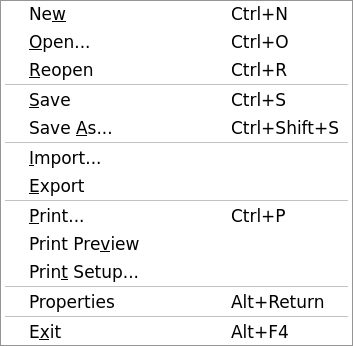
\includegraphics[width=\textwidth]{images/menu-File.png}\end{minipage}\hfill
\begin{minipage}[t]{0.58\textwidth}\vspace{0pt}
\begin{itemize}[leftmargin=1em]
  \item \menu{New}, \menu{Open\ldots}, \menu{Reopen} (loads the song from the last saved version), \menu{Save}, \menu{Save As\ldots}:
        the song is an \texttt{.rmt} file; \texttt{.txt} and \texttt{.rmw} are chosen in the file type of the dialog.
  \item \menu{Import\ldots}: ProTracker modules and TMC songs (chapter~\ref{ch:importexport}).
  \item \menu{Export}: the formats for the Atari (chapter~\ref{ch:importexport}).
  \item \menu{Print}, \menu{Print Preview}, \menu{Print Setup}: the screen of the song is printed on a landscape page, scaled to fill it.
  \item \menu{Properties} (\key{ALT+ENTER}): the properties of the song.
\end{itemize}
\end{minipage}

\section{Edit}

\begin{minipage}[t]{0.5\textwidth}\vspace{0pt}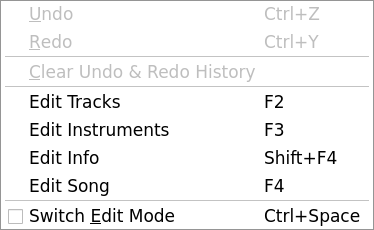
\includegraphics[width=\textwidth]{images/menu-Edit.png}\end{minipage}\hfill
\begin{minipage}[t]{0.46\textwidth}\vspace{0pt}
Undo and redo (the history can be cleared), the four parts of the screen (tracks, instruments, info, song), and the switch between
edit and prove mode.
\end{minipage}

\section{View}

\begin{minipage}[t]{0.36\textwidth}\vspace{0pt}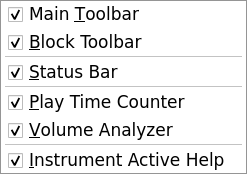
\includegraphics[width=\textwidth]{images/menu-View.png}\end{minipage}\hfill
\begin{minipage}[t]{0.6\textwidth}\vspace{0pt}
Shows or hides the toolbars and the status bar, the play time counter, the volume analyzer and the instrument active help. The
choices are kept in the configuration.
\end{minipage}

\section{Play}

\begin{minipage}[t]{0.5\textwidth}\vspace{0pt}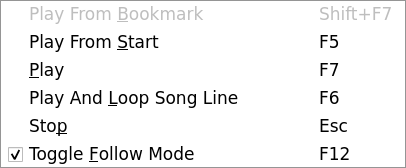
\includegraphics[width=\textwidth]{images/menu-Play.png}\end{minipage}\hfill
\begin{minipage}[t]{0.46\textwidth}\vspace{0pt}
Play from the bookmark, from the start, from the cursor, loop the song line, stop and follow mode (chapter~\ref{ch:playing}).
\end{minipage}

\section{Channels}

\begin{minipage}[t]{0.5\textwidth}\vspace{0pt}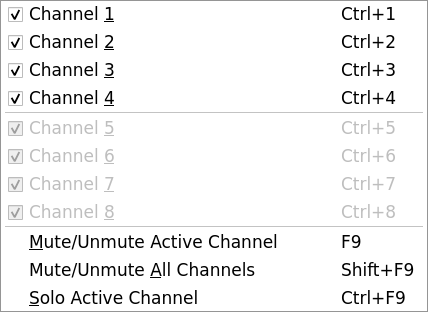
\includegraphics[width=\textwidth]{images/menu-Channels.png}\end{minipage}\hfill
\begin{minipage}[t]{0.46\textwidth}\vspace{0pt}
Switch on and off each of the channels 1 to 8, mute or unmute the active one or all of them, or play the active one alone.
\end{minipage}

\section{Song}

\begin{minipage}[t]{0.58\textwidth}\vspace{0pt}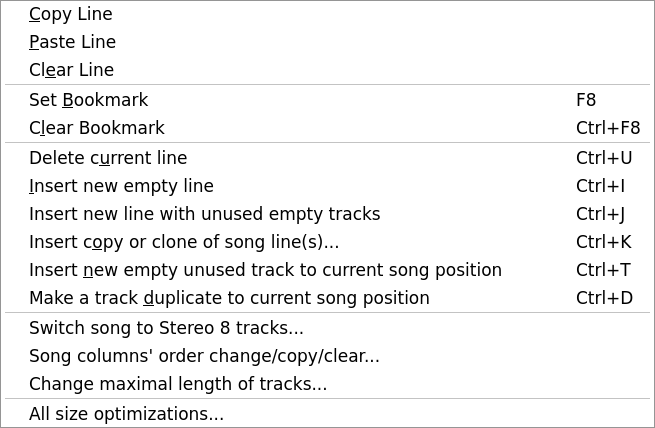
\includegraphics[width=\textwidth]{images/menu-Song.png}\end{minipage}\hfill
\begin{minipage}[t]{0.38\textwidth}\vspace{0pt}
Copy, paste and clear a song line; the bookmark; insert and delete lines; insert tracks; and the commands of chapter~\ref{ch:song}
that change the whole song.
\end{minipage}

\section{Instrument}

\begin{minipage}[t]{0.5\textwidth}\vspace{0pt}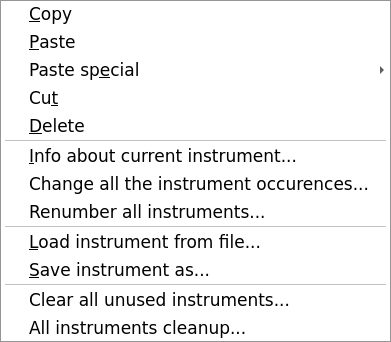
\includegraphics[width=\textwidth]{images/menu-Instrument.png}\end{minipage}\hfill
\begin{minipage}[t]{0.46\textwidth}\vspace{0pt}
Everything to do with an instrument: copy and paste (and paste special), information, change or renumber, clear the unused ones,
load and save (chapter~\ref{ch:instruments}).
\end{minipage}

\section{Track}

\begin{minipage}[t]{0.58\textwidth}\vspace{0pt}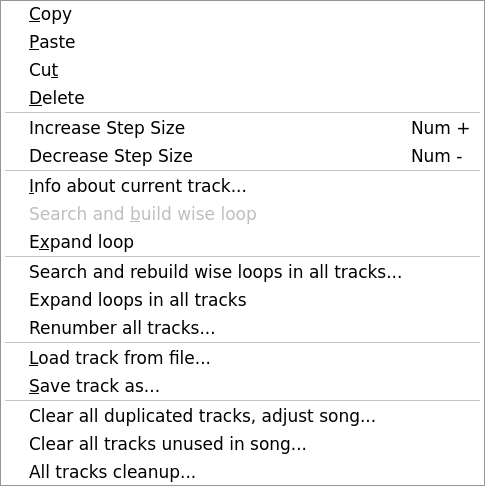
\includegraphics[width=\textwidth]{images/menu-Track.png}\end{minipage}\hfill
\begin{minipage}[t]{0.38\textwidth}\vspace{0pt}
Copy, paste, cut and delete a track; the step size; information about the current track; wise loops; renumbering; loading and saving a
track; and the clean-up of the tracks of the song.
\end{minipage}

\section{Block}

\begin{minipage}[t]{0.5\textwidth}\vspace{0pt}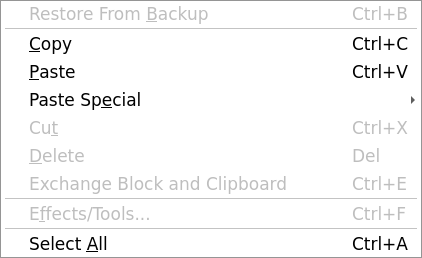
\includegraphics[width=\textwidth]{images/menu-Block.png}\end{minipage}\hfill
\begin{minipage}[t]{0.46\textwidth}\vspace{0pt}
The commands of the blocks (chapter~\ref{ch:tracks}): restore from the backup, copy, paste, paste special (merge, only the volumes, only the
speeds), cut, delete, exchange, effects and tools, select all.
\end{minipage}

\section{Pokey}

\begin{minipage}[t]{0.58\textwidth}\vspace{0pt}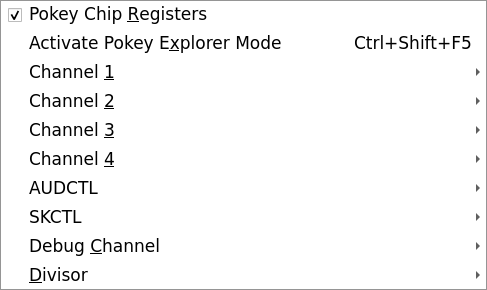
\includegraphics[width=\textwidth]{images/menu-Pokey.png}\end{minipage}\hfill
\begin{minipage}[t]{0.38\textwidth}\vspace{0pt}
The registers of the chip and the Pokey explorer mode, with a submenu for each channel (chapter~\ref{ch:explorer}).
\end{minipage}

\section{Tools}

\begin{minipage}[t]{0.35\textwidth}\vspace{0pt}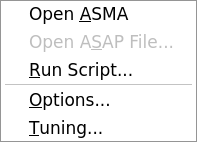
\includegraphics[width=\textwidth]{images/menu-Tools.png}\end{minipage}\hfill
\begin{minipage}[t]{0.61\textwidth}\vspace{0pt}
\menu{Open ASMA} opens the Atari SAP Music Archive in the browser; \menu{Run Script\ldots} runs a script
(chapter~\ref{ch:scripting}); \menu{Options\ldots} and \menu{Tuning\ldots} open the dialogs of chapter~\ref{ch:options}.
\end{minipage}

\section{Help}

\begin{minipage}[t]{0.32\textwidth}\vspace{0pt}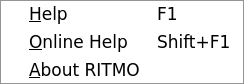
\includegraphics[width=\textwidth]{images/menu-Help.png}\end{minipage}\hfill
\begin{minipage}[t]{0.64\textwidth}\vspace{0pt}
\menu{Help} (\key{F1}) opens this manual, and \menu{Online Help} (\key{SHIFT+F1}) the reference of the original
\RMT{} (menus, keys, instruments), both in the browser, from the GitHub page of \RITMO{} (they need the Internet).
\menu{About RITMO} shows the version and the credits; on a small screen, or with large fonts, its text scrolls.
\end{minipage}

\chapter{Options and tuning}\label{ch:options}

\section{The Options dialog}\label{sec:options}

\menu{Tools $\rightarrow$ Options\ldots} opens the dialog of figure~\ref{fig:dialog-options}. The settings are saved when the
program closes, in the settings of the system (chapter~\ref{ch:install}).

\dialog{dialog-options}{The \menu{Options} dialog.}{9.5cm}

\subsection{General}

\begin{description}[style=nextline,leftmargin=1.2cm]
  \item[Interface size (in \%)] The size of the drawing of the window, from 100\% to 300\%. Only whole multiples of 100\% keep
        the pixels exact. The first start chooses it from the size of the screen (section~\ref{sec:window}).
  \item[Track line highlight step] The two numbers of the \texttt{HIGHLIGHT} field of the info area: every how many lines the lines of
        the tracks are highlighted (for example 8 and 4).
  \item[Use German notation] The note \texttt{B} is written \texttt{H}, as in the German notation.
  \item[Alternative track line numbering] The line numbers follow the highlight step.
  \item[Display accidentals as flats instead of sharps] \texttt{D\#} is written as \texttt{Eb}.
  \item[Audio buffer] How much sound the output of the system takes at a time, from 5 to 40 milliseconds. A small buffer
        makes the sound follow the keys and the MIDI keyboard sooner; a larger one keeps the sound clean when the computer or
        the sound server is busy. The default is 20\,ms on Linux, where the sound servers (PipeWire, PulseAudio) work in
        pieces of about that size, and 5\,ms on Windows and macOS. The output keeps about three buffers of sound ready (60\,ms
        with the 20\,ms buffer), so that a short stall of the sound server is not heard as a gap. If the sound crackles or is
        distorted, choose 30 or 40\,ms.
  \item[Smooth scroll during playback] The lines of the tracks scroll one pixel at a time while a song plays.
  \item[Debug display] A line of internal values in the status bar, off by default. Enable it only if you know what it shows.
\end{description}

The video standard and the tracker driver are not here: they belong to the module, and are set in its properties
(section~\ref{sec:module-properties}).

\subsection{Keyboard}

\begin{description}[style=nextline,leftmargin=1.2cm]
  \item[Keyboard layout] QWERTY, QWERTZ or AZERTY: where the piano of the note keys is. The first start picks the layout from the
        language of the keyboard.
  \item[Move to previous/next song line while track boundaries are crossed] The cursor passes from the end of a track to the next
        song line, and the other way round.
  \item[Remember octaves and volumes separately for each instrument] Each instrument keeps the octave and the volume you last used with it.
  \item[Reset the Atari sound routines each time ESC is pressed] \key{ESC} also starts the player routine again.
  \item[Prompt a save dialog box each time CTRL+S is pressed] \key{CONTROL+S} asks where to save, also from the menu and the
        toolbar.
\end{description}

\subsection{MIDI}

The MIDI input device, the touch response, the Atari volume offset and \emph{Record note off}: they are described in
chapter~\ref{ch:midi}.

\subsection{Paths}

The \menu{Paths\ldots} button opens a dialog with the default folders of the songs, the instruments and the tracks, each with a
\menu{Browse} button. The dialogs to open and save start there.

\section{The module properties}\label{sec:module-properties}

\menu{File $\rightarrow$ Properties\ldots} (\key{ALT+ENTER}) opens the dialog of figure~\ref{fig:dialog-module-properties}: what the
module holds (the file, the channels, the speeds, the instruments and tracks used, the size of the RMT module), then the settings that
belong to the module rather than to the program. They are saved with the other settings when the program closes.

\dialog{dialog-module-properties}{The \menu{Module Properties} dialog.}{9.5cm}

\begin{description}[style=nextline,leftmargin=1.2cm]
  \item[NTSC system speed (60 Hz)] The video system of the song: 60 frames a second instead of the 50 of PAL. The same switch is
        \key{CONTROL+F12}.
  \item[RMT Driver Version] The tracker driver, the player routine that makes the sound while you work (chapter~\ref{ch:drivers}). The
        driver must be the one the song was made with; the default is \emph{RMT 1.34 Patch16 by VinsCool}. The driver chosen here is
        also the one new and opened songs start with. A song that uses the Autofilter, opened with the RMT 1.28 Unpatched driver at
        its question, plays with that driver for itself only: the dialog says so, and the default stays as it was.
  \item[Tuning\ldots] The tuning of section~\ref{sec:tuning}. The button is enabled only for \emph{RMT 1.34 Patch16}, the only
        driver whose frequency tables the tuning reaches: the others play the tables inside their player.
\end{description}

\section{The tuning}\label{sec:tuning}

\menu{Tools $\rightarrow$ Tuning\ldots} (figure~\ref{fig:dialog-tuning}) is a calculator for the pitch of the notes. The POKEY makes its
frequencies by dividing a clock, so not every pitch exists: the program computes the divisors that come nearest to the notes of
the temperament you choose, and the tracker plays with them.

\dialog{dialog-tuning}{The \menu{Tuning} dialog.}{10cm}

\begin{description}[style=nextline,leftmargin=1.2cm]
  \item[Base tuning (Hz) and Base note] The frequency of a reference note, by default \texttt{A-} at 440.8375\ldots\,Hz. It can be any
        number: \texttt{432}, \texttt{443.9}\ldots
  \item[Temperament] \emph{Equal Temperament} (the default) or another. The \emph{Ratio} table lists the interval of each step over the unison
        as a fraction.
  \item[Reset] puts the default values back; \menu{Test now} tries the tuning.
\end{description}

The tuning is saved with the configuration and is also the one a script uses when it exports a song (chapter~\ref{ch:scripting}).

\chapter{Import and export}\label{ch:importexport}

\section{Importing}

\menu{File $\rightarrow$ Import\ldots} reads a ProTracker module (\texttt{.mod}) or a TMC song (\texttt{.tmc}, \texttt{.tm8}) and
makes a song of it. After the file is chosen the dialog of figure~\ref{fig:dialog-import} asks how to convert a module.

\dialog{dialog-import}{Importing a ProTracker module.}{11cm}

\begin{itemize}
  \item The \emph{type of RMT module}: \texttt{RMT4} (the four channels of the module on the four tracks) or \texttt{RMT8}
        (the channels spread on the two POKEYs, in the order 1, 4 / 2, 3).
  \item The treatment of the \emph{notes} (shift the octave down if the tuning of the song is too high, replace the portamento
        effects by calculated notes), of the \emph{volumes}, and the \emph{size optimizations} that are made while importing (wise loops, cutting
        the unused parts of the tracks).
\end{itemize}

When the conversion is done a dialog reports how many tracks, instruments and song lines the song has, and what the optimizations did.
Check the box and press \menu{OK}: the song is loaded, but it still needs your work. The instruments are rough: look at their envelopes and
distortions (drums, basses\ldots) and correct the tunings of the original samples.

\dialog{dialog-import-2}{The result of the import.}{9cm}

\section{Exporting}

\menu{File $\rightarrow$ Export} writes the song in a format for the Atari. The file dialog chooses the name and the format; most of the
formats then show a dialog of options. Every format is written from the data of the song as the tracker plays it.

\begin{center}
\begin{tabular}{@{}>{\raggedright\arraybackslash}p{4.2cm}p{9.6cm}@{}}
\toprule
Format & Use \\ \midrule
RMT stripped song file (\texttt{.rmt}) & the module without the names and the unused tracks and instruments, to link in a program that uses
  the RMT player routine \\
ASM simple notation (\texttt{.asm}) & the notes as assembler data, for your own player \\
SAP-R data stream (\texttt{.sapr}) & the register writes of the POKEY, frame by frame \\
Compressed SAP-R (\texttt{.lzss}) & the same, compressed, for the LZSS player \\
SAP file + LZSS driver (\texttt{.sap}) & a file the Atari players (ASAP, the plug-ins of many players, ASMA) play directly \\
XEX Atari executable (\texttt{.xex}) & a program for the Atari that plays the song when it is started \\
XEX Atari executable + RMT player (\texttt{.xex}) & the same with the RMT player and the module of the song \\
Relocatable ASM for RMTPlayer (\texttt{.asm}) & the module as source with labels, to be placed in memory by your program \\
WAV audio file (\texttt{.wav}) & the sound as a 16-bit, 44.1\,kHz, stereo file, the song played once up to its loop \\
\bottomrule
\end{tabular}
\end{center}

\subsection{RMT stripped}

\dialog{dialog-export-stripped-rmt}{The export of an RMT stripped file.}{10cm}

The \emph{from address} is where the module will be in the memory of the Atari; the program shows the range it takes. The
options are \emph{SFX support} (keep the unused tracks and instruments, for sound effects played by the game),
\emph{GlobalVolumeFade} (a variable the program can use to fade the music) and \emph{No songline start} (the song always starts from
song line 0). The text box lists the \emph{RMT FEATures} the song uses: if a game uses only this song, these definitions can be pasted into
the player routine source (\texttt{rmt\_feat.a65}), which then assembles to a smaller and faster routine
(this is described in the file \texttt{optimization.txt} that comes with the program).

\subsection{ASM simple notation}

\dialog{dialog-export-simple-asm}{The export of the notes as assembler data.}{8cm}

Choose what to export (the tracks, or the whole song by song columns), how the note is written (the index \texttt{\$00}--\texttt{\$3C}, or the
frequency according to the distortion of the instrument), how the duration is written (notes only, with the special value
\texttt{XXX} in empty beats, or pairs of note and duration, in either order) and the prefix of the labels (empty for none).

\subsection{SAP, SAP-R and LZSS}

\dialog{dialog-export-sap}{The export of a SAP file.}{8cm}

A SAP file has a header with the name, the author and the date, which the dialog fills with those of the song. The field
\emph{Subsongs} lists, in hexadecimal, the song line each subsong starts from: \texttt{00} for one tune, \texttt{00 10} for two. SAP-R is the stream of
the POKEY registers; LZSS compresses it, and the SAP file contains it with the player routine of the VU-Player.

In the SAP file each subsong plays its intro once and then its loop for ever, at full volume. The SAP files of RITMO before 2.6 did
not: at the second end of the loop the player started a fade out that stopped after one step, so from the third pass on the song
played one volume step lower and one frame early.

\subsection{XEX}

\dialog{dialog-export-xex}{The export of an Atari executable.}{10cm}

The program an XEX file contains shows a text on the Atari screen while it plays: up to five lines of 40 characters (the fifth shown
instead of the fourth when the \key{SHIFT} key of the Atari is held down). Below, the \emph{rasterbar} shows the CPU usage of the player
in colour, \emph{shuffle} changes its colours, and the box \emph{Automatically adjust playback speed}, with the line that says that the speed will be
adjusted to 50\,Hz on both PAL and NTSC systems, turns the adjustment of the speed on. The preview shows
the text as the Atari will draw it.

\subsection{XEX with the RMT player}

\dialog{dialog-export-xex-rmt}{The export of an Atari executable with the RMT player.}{8cm}

This XEX holds the RMT player and the module of the song, not the stream of the POKEY registers: the file is
smaller, a long song or a stereo song at a high instrument speed fits, and the Atari computes the music as the tracker does.
The player is the one of the tracker driver: RMT~1.28 for \emph{RMT 1.28 Unpatched}, Patch16 for \emph{RMT 1.34 Patch16}, with
the frequency tables of the tuning in use. With the other drivers there is no player and the export stops with a message.

The dialog asks for the three lines the program shows, NAME, AUTHOR and DATE (up to 200 characters each; a line
longer than the 40 characters of the screen scrolls). It proposes them from the name of the song, as the tracker writes it:
the name up to its first comma, the rest, and the first year it mentions.

\dialog{atari-rmtplay}{RITMO PLAYER on the Atari, with the stereo reference song.}{10cm}

On the Atari, RITMO PLAYER (the visualizer of RMTPLAY of VERA\_ATARI\_PBI) shows the three lines, one volume bar per
channel, the POKEY registers, the song line, the row, the speed and the play time; \key{SPACE} pauses, \key{R} starts the
song again and \key{ESC} goes back to DOS. An 8-track song plays on two POKEYs, with eight bars. The instrument speed (1 to
4) is the number of calls of the player in every frame; a song for the other region (PAL or NTSC) plays at its own speed.
The module goes after the program, up to \texttt{\$B820}: about 24\,KB; a bigger one stops the export with a message.

\subsection{Relocatable ASM}

\dialog{dialog-export-reloc-asm}{The export of a relocatable module.}{10cm}

The module is written as byte definitions with labels (the one of the start of the song data, and optionally separate labels for the
instruments, the tracks and the song lines, which can be placed in different places of memory). The text box shows the size of each
part and the order of the modules.

\subsection{WAV}

The WAV export has no options: it plays the song with the built-in emulation and writes the sound.

\section{Exporting from the command line}

All the formats can be exported from a script, with no window, so that the files of a release are made from the \texttt{.rmt}
source (chapter~\ref{ch:scripting}).

\input{chapters/13-midi.tex}
\chapter{The Pokey explorer}\label{ch:explorer}

The explorer is a mode to study the sound of the POKEY. \menu{Pokey $\rightarrow$ Activate Pokey Explorer Mode}
(\key{CONTROL+SHIFT+F5}) stops the tracker's player routine and lets the keys write the registers of the chip directly, so that you can hear
the effect of each divisor, distortion and \texttt{AUDCTL} bit. The mode is left with the edit/jam toggle (\key{CONTROL+SPACE}).

\shot{window-explorer}{The Pokey explorer mode, with the registers of the chip on the screen.}{0.98}

With \menu{Pokey $\rightarrow$ Pokey Chip Registers} on, three rows under the dumps of the registers detail one channel: its \texttt{AUDF} and
\texttt{AUDC} bytes, the first divisor of \texttt{AUDF + MODOFFSET} from 3 up (\texttt{MODULO}), the coarse divisor of the pitch formula (28 at
64\,kHz, 114 at 15\,kHz, 1 at 1.79\,MHz and for joined channels), the free divisor, the modulo offset (1, 4 at 1.79\,MHz, 7 for joined channels)
and the resulting pitch.

\section{The keys}

The keys are the physical positions of the QWERTY layout (on QWERTZ and AZERTY they are the keys at the same positions).

\begin{center}
\begin{tabular}{@{}lp{10.5cm}@{}}
\toprule
Key & Function \\ \midrule
\key{ENTER} / \key{BACKSPACE} & next / previous channel (0--3) \\
\key{+} / \key{-} & divisor $+0.1$ / $-0.1$; with \key{SHIFT} $+1.0$ / $-1.0$ (from 1.0 to 10000.0) \\
\key{1} \key{3} \key{5} \key{7} & \texttt{AUDF0} to \texttt{AUDF3} $+1$; with \key{SHIFT} $+\$10$ \\
\key{Q} \key{E} \key{T} \key{U} & \texttt{AUDF0} to \texttt{AUDF3} $-1$; with \key{SHIFT} $-\$10$ \\
\key{2} \key{4} \key{6} \key{8} & \texttt{AUDC0} to \texttt{AUDC3} $+1$; with \key{SHIFT} $+\$10$ \\
\key{W} \key{R} \key{Y} \key{I} & \texttt{AUDC0} to \texttt{AUDC3} $-1$; with \key{SHIFT} $-\$10$ \\
\key{C} \key{G} \key{F} \key{K} \key{J} \key{D} \key{A} \key{P} & toggle the bits 0 to 7 of \texttt{AUDCTL}: the 15\,kHz clock, the two high pass filters, the
  two 16-bit joins, the two 1.79\,MHz clocks and the 9-bit poly counter \\
\key{M} & toggle the two-tone bits of \texttt{SKCTL} \\
\bottomrule
\end{tabular}
\end{center}

The \menu{Pokey} menu has the same operations as menu items, which work in the explorer mode only.

\input{chapters/15-drivers.tex}
\input{chapters/16-scripting.tex}

\appendix
\input{chapters/a-reference.tex}
\input{chapters/b-format.tex}
\input{chapters/c-midi-chart.tex}
\chapter{Building from the source}\label{app:building}

\RITMO{} is built with CMake and Qt. The full instructions are in the file \texttt{BUILD.md} of the source; here is the short version.

\section{Linux}

\begin{lstlisting}
sudo apt install cmake qt6-base-dev portaudio19-dev librtmidi-dev
cmake -B build-qt -DCMAKE_BUILD_TYPE=Release
cmake --build build-qt -j
./build-qt/out/ritmo song.rmt
\end{lstlisting}

The program is \texttt{build-qt/out/ritmo}, with the \texttt{resources} folder next to it. It needs Qt~6: Qt~5 is no longer
supported from 2.6.

\section{Windows and macOS}

Windows is built with MSYS2 (MinGW64: GCC, Qt~6, PortAudio, RtMidi) and macOS with the Apple compiler and the Qt of the official installer. The
GitHub workflows of the repository (\texttt{.github/workflows}) build the packages of both, and the AppImage for Linux
(\texttt{scripts/build-appimage.sh}), and are the best description of the steps.

\section{Linux riscv64 and ppc64}

There is no AppImage for these architectures (no official Qt~6, no \texttt{linuxdeploy}). The workflow
\texttt{.github/workflows/build-linux-ports.yml} builds the program in a Debian container of the architecture emulated by QEMU:
\texttt{debian:trixie} for riscv64, a \texttt{debootstrap} of Debian ports \emph{sid} for ppc64. Two scripts do the work, and can be
started by hand in any Debian of the architecture:
\begin{lstlisting}
docker run --rm --platform linux/riscv64 -v "$PWD":/src -w /src debian:trixie \
    sh -c 'scripts/build-tarball.sh && scripts/build-deb.sh'
\end{lstlisting}
\texttt{scripts/build-tarball.sh} makes the \texttt{.tar.gz} with the libraries (\texttt{lib}, \texttt{plugins}) and the launcher;
\texttt{scripts/build-deb.sh} makes the \texttt{.deb}, whose dependencies come from \texttt{dpkg-shlibdeps}. Both run the program
without a display as a test.

The engine on PowerPC 64 big endian is tested on every push (\texttt{.github/\allowbreak workflows/\allowbreak test-\allowbreak bigendian.yml}):
\texttt{RmtCoreTest} is built for x86\_64 and cross-compiled for ppc64, run by \texttt{qemu-ppc64}, and
\texttt{scripts/test-endian.sh} compares the POKEY registers, the sound and the screen of every song of \texttt{rmt/songs}.

\section{Core only and tests}

\texttt{-DRMT\_BUILD\_CORE\_ONLY=ON} builds the engine and the audio and MIDI backends without Qt, and with \texttt{-DRMT\_CORE\_TEST=ON}
the \texttt{RmtCoreTest} program, a smoke test of the engine. The \texttt{scripts/test-scripting.sh} script runs the reference scripts.

\section{Test hooks}

For tests and documentation the program can run without a display (\texttt{QT\_QPA\_PLATFORM=offscreen}). The environment variables
\texttt{RMT\_QT\_GRAB} (save the window and quit), \texttt{RMT\_QT\_KEYS}, \texttt{RMT\_QT\_COMMANDS}, \texttt{RMT\_QT\_FILEDIALOG},
\texttt{RMT\_QT\_DIALOG} and \texttt{RMT\_QT\_MENU\_GRAB} (the menus as images) press keys, run menu commands, answer the dialogs and save them;
\texttt{RMT\_QT\_FONT} fixes the font of the menus and of the dialogs, so that the images do not depend on the desktop. The
screenshots of this manual were taken that way, by \texttt{doc/manual/make-screenshots.sh}.

\input{chapters/e-credits.tex}

\end{document}
